%!TEX TS-program = xelatex
\documentclass[mathserif, aspectratio=169]{beamer}

\usetheme{Warsaw}
\usetheme[progressbar=frametitle]{metropolis} % 이 행을 주석처리하면 Warsaw 테마가 적용됨.
\usepackage{kotex}
\usepackage{ragged2e}
\usepackage{multicol}
\usepackage{verbatim}
\usepackage{amsmath}
\usepackage{graphics}
\usepackage{setspace}
\usepackage{wrapfig}
\usepackage{hyperref}

\title{인터넷 기사의 댓글 속 혐오 양상에 대하여}
\setbeamerfont{title}{series=\bfseries}

\author{20205178 박~~현\hfill 인공지능 알고리즘을 이용한 사회과학연구 -- 기말 프로젝트}
\setbeamerfont{author}{size=\scriptsize, series=\bfseries}
\institute{}
\date{}

\setbeamertemplate{navigation symbols}{}
% \setbeamerfont{frametitle}{series=\bfseries,parent=structure}

\setbeamertemplate{itemize/enumerate body begin}{\normalsize}
\setbeamertemplate{itemize/enumerate subbody begin}{\footnotesize}
\setstretch{1.25}



\begin{document}
\frame{\titlepage}
\metroset{sectionpage=none}
\metroset{block=fill}

\section{주제 선정 이유}
\begin{frame}
    \frametitle{주제 선정 이유}
    \justifying
    최근 온 $\cdot$ 오프라인 상에서의 혐오가 사회적 문제로 떠오르고 있다.
    이에 수 년간의 인터넷 기사 댓글을 수집하여 Smilegate AI에서 공개한 \href{https://github.com/smilegate-ai/korean_unsmile_dataset}{Korean UnSmile Dataset}에서 제공하는 인공지능 모델을
    이용하여 각 댓글에 해당하는 혐오 분류를 찾아 이들에 대한 분포 및 양상을 분석하고자 한다.
\end{frame}
\section{알고리즘 적용 과정}
\begin{frame}
    \frametitle{사용한 패키지 -- GNU S}
    \begin{description}[labelwidth=3cm]
        \item [future:] Unified Parallel and Distributed Processing in R for Everyone
        \item [future.apply:] Apply Function to Elements in Parallel using Futures
        % \item [reticulate:]  Interface to `Python'
        \item [rvest:] Easily Harvest (Scrape) Web Pages
        \item [tidyverse:] Easily Install and Load the `Tidyverse'
        \item [RmecabKo:] Rcpp Wrapper for Eunjeon Project
        \item [plotly:] Create Interactive Web Graphics via `plotly.js'
        \item [wordcloud2:] Create Word Cloud by `htmlwidget'
        \item [sqldf:] Manipulate R Data Frames Using SQL
        \item [httr:] Tools for Working with URLs and HTTP
        % \item [reshape2:] Flexibly Reshape Data: A Reboot of the Reshape Package
    \end{description}
\end{frame}
\begin{frame}{사용한 패키지 -- Python}
    \begin{description}[labelwidth=3cm]
        \item [Hugging Face:] Datasets, Transformers.
        \item [Pandas:] Python Data Analysis Library
        \item [flask:] A simple framework for building complex web applications.
    \end{description}
\end{frame}
\begin{frame}{자료 수집}
    \includegraphics[width = \linewidth]{images/data_scrap.pdf}
\end{frame}
\begin{frame}{감정 분석}
    \begin{columns}
        \begin{column}{0.3\linewidth}
            \centering
            \includegraphics[width = 0.8\linewidth]{images/sentiment_analysis.pdf}
        \end{column}
        \begin{column}{0.7\linewidth}
            \begin{enumerate}
                \item SQLite로부터 수집한 댓글을 가져오기.
                \item 댓글마다 R의 \texttt{httr::POST(url)}을 이용하여 도커 내 REST API 서버에 POST 요청을 보냄.
                \item Docker 안에서 BERT 모델을 이용해 감정 분석을 GPU로 가속하며 진행.
                \item R에서 감정 분석 결과들을 \texttt{do.call(rbind, dfs)}를 이용해 병합.
            \end{enumerate}
        \end{column}
    \end{columns}
\end{frame}
\begin{frame}{시각화 -- 꺽은선 그래프}
    \begin{columns}
        \begin{column}{0.5\linewidth}
            \centering
            \begin{figure}
                \includegraphics[width = \linewidth]{images/lineplot.pdf}
            \end{figure}
        \end{column}
        \begin{column}{0.5\linewidth}
            \begin{itemize}
                \item clean과 악플의 비율은 비슷하다.
                \item 남성과 여성의 양상이 유사하다.\\$\rightarrow$ 상관분석을 해보자.
            \end{itemize}
        \end{column}
    \end{columns}
\end{frame}
\begin{frame}{시각화 -- 레이더 차트}
    \begin{columns}
        \begin{column}{0.5\linewidth}
            \centering
            \begin{figure}
                \includegraphics[width = \linewidth]{images/radarchart.pdf}
            \end{figure}
        \end{column}
        \begin{column}{0.5\linewidth}
            \justifying
            \begin{itemize}
                \justifying
                \item 여러 분류에 대한 분포를 쉽게 볼 수 있는 레이더 차트를 이용하여 시각화해보았다.
                \item clean과 악플이 다른 분류에 비해 매우 높아 보기 어려워 시연 파트에서 인터랙티브한 그래프를 보여주며 살펴보고자 한다.
            \end{itemize}
        \end{column}
    \end{columns}
\end{frame}
\begin{frame}{시각화 -- 히트 맵}
    \begin{columns}
        \begin{column}{0.5\linewidth}
            \centering
            \begin{figure}
                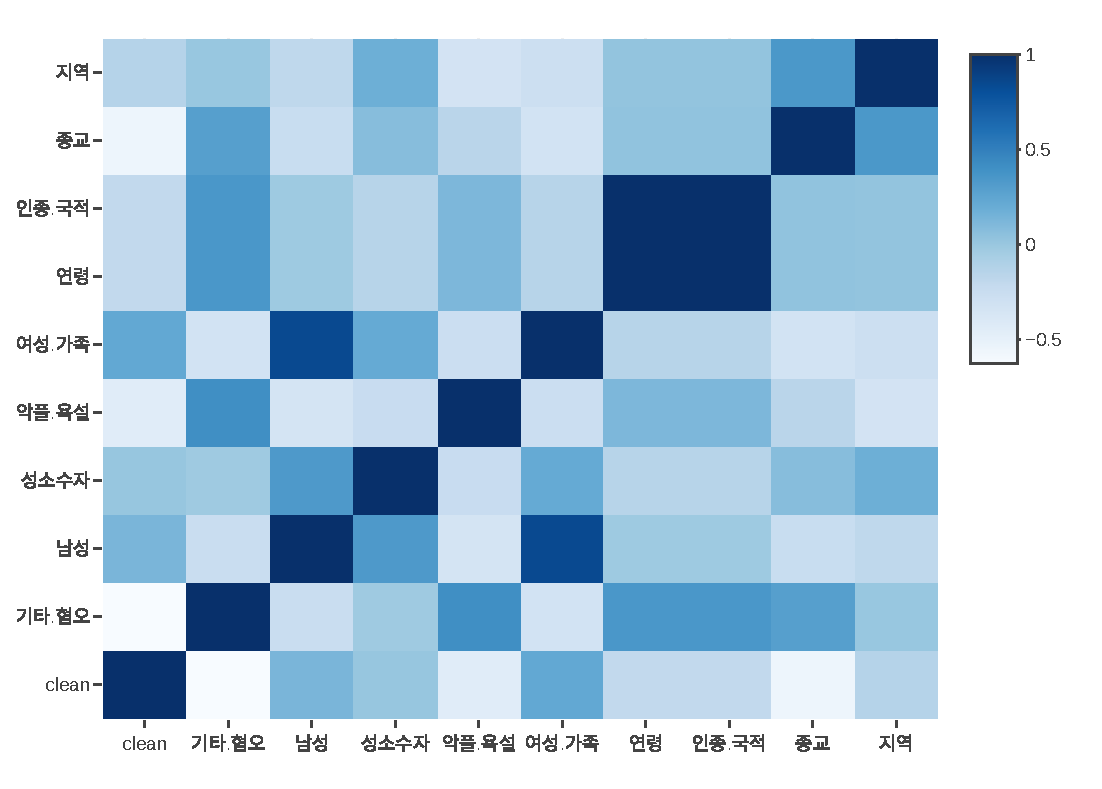
\includegraphics[width = \linewidth]{images/heatmap.pdf}
            \end{figure}
        \end{column}
        \begin{column}{0.5\linewidth}
            \justifying
            \begin{itemize}
                \justifying
                \item \texttt{cor(df)}를 이용하여 상관계수를 구한 결과를 히트 맵을 이용하여 시각화해보았다.
                \item 위에서 꺽은선 그래프를 통해 확인한 바와 같이 남성과 여성의 상관관계가 매우 높다는 사실을 알 수 있다.
                \item 그 외에도 지역과 종교 간의 상관성과 남성과 성소수자 간의 상관성 또한 높음을 히트 맵을 통해 확인할 수 있었다.
            \end{itemize}
        \end{column}
    \end{columns}
\end{frame}
\section{함의}
\begin{frame}{결과}
    \justifying
    \textbf{감정 분석}\\
    악플과 그렇지 않은 댓글의 비율은 비슷했다.\\~\\
    \textbf{상관 분석}\\
    여성에 대한 혐오와 남성에 대한 혐오가 매우 큰 상관성을 갖는 것으로 나왔으며, 
    종교와 지역 간의 상관성과 남성과 성소수자 간의 상관성 또한 다른 요소에 비해
    높은 것으로 나타났다.\\
\end{frame}
\section{코드}
\begin{frame}{코드 -- 웹 스크래핑}
    \begin{columns}
        \begin{column}{0.5\linewidth}
            \centering
            \begin{figure}
                \includegraphics[scale = 0.12]{images/codes/get_news_list.png}
            \end{figure}
        \end{column}
        \begin{column}{0.5\linewidth}
            \centering
            \begin{figure}
                \includegraphics[scale = 0.12]{images/codes/get_news_comments.png}
            \end{figure}
        \end{column}
    \end{columns}
\end{frame}
\begin{frame}{코드 -- 워드 클라우드}
    \begin{columns}
        \begin{column}{0.5\linewidth}
            \centering
            \begin{figure}
                \includegraphics[scale = 0.12]{images/codes/wordcloud.png}
            \end{figure}
        \end{column}
        \begin{column}{0.5\linewidth}
            \justifying
            SQL를 이용하여 데이터를 가공해 데이터 프레임으로 가져와
            tidyverse에 있는 여러 함수를 이용해 필요에 맞게 다시 한 번 가공한 후
            \texttt{RmecabKo::nouns} 함수를 이용하여 명사를 추출해
            워드 클라우드를 그리는 코드.
        \end{column}
    \end{columns}
\end{frame}
\begin{frame}{코드 -- GitHub}
    \centering
    프로젝트을 진행하며 작성한 모든 코드는 아래 저장소에 전부 업로드 되어 있습니다.\\~\\~\\
    \href{https://github.com/HyunP-dev/Social-Science-Study-using-AI-Final-Project/}
         {https://github.com/HyunP-dev/Social-Science-Study-using-AI-Final-Project/}
\end{frame}
\begin{frame}
    \centering
    \Huge{-- Demonstration --}
\end{frame}
\end{document}